% ---------------------------------------------------------------------------
\FloatBarrier
\section{Physics-Informed Features (RQ3, Part 1)}
\label{sec:physics}

This phase designs the fourth feature set, F4, from the degradation
mechanisms. With 41 training cells, a few well-founded features are worth more
than many weak ones, because every weak feature is another chance to overfit.
Every candidate was therefore screened against five criteria, using the
\emph{training cells only}; the test sets are first used in the model
comparison (Phase~4). The screening is implemented in
\texttt{src/screen\_physics.py} and shown step by step in
\texttt{notebooks/03\_physics\_features.ipynb}.
\begin{enumerate}
  \item A physical mechanism behind the feature.
  \item Information beyond $\log_{10}\mathrm{Var}(\dq)$: the $t$-statistic of
  the candidate in a regression of $\log_{10}$(life) on $\log_{10}\mathrm{Var}(\dq)$
  and the candidate, fitted within each batch, and the paired
  cross-validated gain (4-fold, 100 repeats).
  \item The same sign within each training batch (\texttt{b1} and
  \texttt{b2}); otherwise the feature only identifies the batch.
  \item A gain that remains on top of a plain batch label.
  \item A signal above the measurement noise within cycles $\le 100$.
\end{enumerate}

\subsection{What $\dq$ does not answer}
$\dq$ answers one question well: \emph{how fast is the cell's voltage
curve changing?} Its amplitude is a degradation \emph{rate}. Life, however,
also depends on two things that a rate cannot tell.
\begin{enumerate}
  \item \textbf{How much room is left before end of life?} End of life is a
  fixed capacity, 0.88\,Ah. A cell that starts at 1.094\,Ah has 214\,mAh to
  lose; one that starts at 1.048\,Ah has 168\,mAh, about 20\,\% less (the
  range over the training cells). At the same rate, the second cell reaches
  end of life about 20\,\% sooner.
  \item \textbf{Is the rate itself measured correctly?} Lithium that slowly
  returns from the anode overhang during cycles 10--100 adds charge to the
  later discharge curve and makes $\dq$ look smaller than the degradation
  underneath it.
\end{enumerate}
An analogy: $\dq$ is the fuel consumption of a car. To know how far it will
go, one also needs the fuel left in the tank (question 1), and must correct
the consumption reading for a reserve can that slowly drains into the tank
and makes the consumption look lower than it is (question 2). Features that
describe \emph{which} mechanism is at work (dQ/dV peaks, resistance,
heating) answer neither question, because $\dq$ already integrates the
effect of all mechanisms on the discharge curve. The screening below
confirms this.

\subsection{Screening results}
\label{sec:screen}
Table~\ref{tab:screen} summarises the 19 candidates. Three groups emerge.

\textbf{Mechanism features add nothing beyond $\dq$.} The change in height,
voltage and area of the main dQ/dV peak, the growth of the charge recovered
in the 2.0\,V CV hold, the capacity offset at 2.0\,V, the IR slope against
$\sqrt{N}$ and the temperature rise all \emph{increase} the
cross-validated error when added to $\log_{10}\mathrm{Var}(\dq)$. They are
computed from the same discharge curves, and $\dq$ is already the combined
fingerprint of loss of active material, loss of lithium and kinetics. The
coulombic efficiency cannot be used at all: the median of $Q_D/Q_C$ is
slightly \emph{above} one, so the cycler cannot resolve the small loss per
cycle.

\textbf{Several candidates only identify the batch.} The curvature of the
capacity-fade curve correlates with life at $\rho=+0.53$ over all training
cells, but at $-0.36$ within \texttt{b1} and $+0.39$ within \texttt{b2}
(Simpson's paradox). Over cycles 2--100 capacity first rises (below) and then
falls; in long-lived \texttt{b1} the curvature mostly measures the rise, in
\texttt{b2} it measures fade that has already begun. The plating index of
the policy (mean C-rate between 50 and 80\% SOC), the cell temperature at the
start of the fast charge and the cycle duration also lose or reverse their
correlation within a batch. The temperature integral of the paper's full
model correlates with cycle duration at $r=0.92$ over the training cells.

Table~\ref{tab:steps} breaks the cycle duration into protocol steps. The
\texttt{-newstructure} procedure uses 5-second rests, as in the 2018-04-12
batch~\cite{severson2019}, whereas the 2017-06-30 batch and the standard cells
of the 2018-02-20 batch rest about 10\,min per cycle. Rest time and the cell
temperature at the start of the fast charge line up with the typical life of
each group: a cell that has cooled during the rest is charged fast at a lower
temperature, which favours lithium plating. Within a batch, however, neither
quantity adds information, and rest time is constant within each training
batch, so it cannot be separated from the batch itself. Both are kept as
hypotheses for the unseen-batch analysis rather than used as features.

\textbf{Two features survive}, described next. Both describe what $\dq$
misses rather than a second measurement of what it contains.

\begin{table*}[t]
\centering
\caption{Screening of the physics-informed candidates on the 41 training
cells. $\rho$: Spearman correlation with $\log_{10}$(life); $t$: $t$-statistic
of the candidate given $\log_{10}\mathrm{Var}(\dq)$, fitted within each batch;
gain: change in cross-validated RMSE of $\log_{10}$(life) when the candidate is
added (positive = better), on top of $\log_{10}\mathrm{Var}(\dq)$ and on top of
$\log_{10}\mathrm{Var}(\dq)$ plus a batch label. Bold: selected for F4.}
\label{tab:screen}
\small
\setlength{\tabcolsep}{3pt}
\begin{tabular}{@{}llrrrrrrr@{}}
\toprule
Candidate & Mechanism & $\rho$ all & $\rho$ \texttt{b1} & $\rho$ \texttt{b2} & $t$ \texttt{b1} & $t$ \texttt{b2} & Gain (\%) & Beyond batch (\%) \\
\midrule
dQ/dV peak height change & LAM, LLI & $+0.65$ & $+0.42$ & $+0.44$ & $+0.3$ & $+1.1$ & $-2.4$ & $-1.7$ \\
dQ/dV peak voltage shift & OCV shift, overpotential & $+0.69$ & $+0.53$ & $+0.27$ & $-0.6$ & $+1.6$ & $-3.8$ & $-2.9$ \\
dQ/dV peak area change & capacity of main stage & $+0.77$ & $+0.78$ & $+0.43$ & $-1.6$ & $+2.0$ & $-3.6$ & $-2.6$ \\
$\Delta Q$ at 2.0\,V & LLI & $+0.75$ & $+0.67$ & $+0.29$ & $-2.4$ & $+1.1$ & $-3.4$ & $-15.2$ \\
CV-hold charge growth at 2.0\,V & kinetics & $-0.72$ & $-0.70$ & $-0.31$ & $+1.9$ & $-2.6$ & $-4.1$ & $-4.7$ \\
Coulombic efficiency deficit & side reactions & $+0.12$ & $+0.02$ & $+0.11$ & $+1.4$ & $+0.1$ & $-2.0$ & $-1.1$ \\
IR slope vs.\ $\sqrt{N}$ & SEI growth & $+0.30$ & $-0.39$ & $-0.10$ & $+1.8$ & $-2.8$ & $-1.4$ & $+2.7$ \\
Temperature rise per cycle & Joule heating & $-0.21$ & $-0.32$ & $-0.01$ & $-1.2$ & $+0.8$ & $-1.6$ & $-1.2$ \\
Temp.\ at start of fast charge & plating vs.\ temperature & $+0.54$ & $-0.32$ & $+0.19$ & $-0.4$ & $+2.0$ & $+4.4$ & $-2.0$ \\
Plating index of policy & plating risk & $-0.62$ & $+0.02$ & $+0.03$ & $+0.8$ & $+2.7$ & $-2.7$ & $+7.6$ \\
Curvature of capacity fade & fade acceleration & $+0.53$ & $-0.36$ & $+0.39$ & $+2.9$ & $+1.4$ & $-7.4$ & $-5.5$ \\
Exponent of $\Delta Q$ growth & fade acceleration & $-0.39$ & $-0.23$ & $0.00$ & $-1.4$ & $+0.6$ & $-0.7$ & $+1.9$ \\
Multi-cycle $\Delta Q$ variance & noise reduction & $-0.79$ & $-0.82$ & $-0.33$ & $-2.4$ & $+0.1$ & $-2.6$ & $+2.0$ \\
Cycle of early capacity peak & overhang timing & $+0.20$ & $+0.40$ & $+0.08$ & $-2.3$ & $-2.1$ & $+7.0$ & $+16.8$ \\
Half-rise cycle & overhang timing & $-0.03$ & $+0.32$ & $+0.02$ & $-3.0$ & $-2.3$ & $+17.5$ & $+13.7$ \\
Capacity rise, cycles 2$\to$10 & overhang & $+0.20$ & $+0.46$ & $+0.15$ & $-2.6$ & $-0.7$ & $+6.4$ & $+3.1$ \\
\textbf{Capacity rise after cycle 10} & overhang hiding $\Delta Q$ & $-0.06$ & $+0.42$ & $+0.07$ & $-3.9$ & $-1.6$ & $+25.7$ & $+11.2$ \\
\textbf{Margin / rate} & budget / rate & $+0.83$ & $+0.84$ & $+0.51$ & $+5.3$ & $+0.1$ & $+9.6$ & $-0.3$ \\
Cycle duration & time-based ageing & $-0.69$ & $+0.54$ & $0.00$ & $+0.6$ & $-0.7$ & $+24.8$ & $+2.2$ \\
\bottomrule
\end{tabular}
\end{table*}

\begin{table}[t]
\centering
\caption{Median duration (min) of the protocol steps and cell temperature
at the start of the fast charge, for six random cells per group (cycles 20
and 60). u1-new: \texttt{-newstructure} cells of 2018-02-20.}
\label{tab:steps}
\small
\setlength{\tabcolsep}{3pt}
\begin{tabular}{@{}lrrrrr@{}}
\toprule
Step & \texttt{b1} & \texttt{b2} & \texttt{b3} & \texttt{u1} & u1-new \\
\midrule
Fast charge to 80\% & 11.0 & 10.1 & 10.0 & 10.1 & 10.0 \\
Rest at 80\% SOC & 1.0 & 5.0 & 0.2 & 4.9 & 0.2 \\
1C constant current & 9.4 & 9.0 & 8.9 & 8.3 & 9.0 \\
CV hold at 3.6\,V & 10.5 & 10.9 & 7.9 & 19.7 & 8.8 \\
4C discharge & 14.6 & 14.5 & 14.4 & 14.6 & 14.5 \\
CV hold at 2.0\,V & 5.4 & 5.5 & 3.8 & 7.8 & 4.6 \\
Rest after discharge & 0.0 & 4.9 & 0.1 & 4.9 & 0.2 \\
\midrule
Total & 52.0 & 60.0 & 45.6 & 69.8 & 47.5 \\
$T$ at start of fast charge (\textdegree C) & 32.5 & 31.3 & 35.3 & 31.3 & 33.8 \\
\bottomrule
\end{tabular}
\end{table}

\subsection{Margin to end of life over degradation rate}
Fig.~\ref{fig:p3traj} follows the amplitude (standard deviation) of
$\Delta Q_{n-10}(V)$ for $n=20,30,\ldots,100$. In every cell it follows a power
law in $n-10$ with a median exponent of 1.01 (interquartile range
0.98--1.11, median $R^2=0.986$): the change in the voltage curve grows at a
\emph{constant} rate over the first 100 cycles. The paper hypothesised such
linear degradation for loss of active material~\cite{severson2019}; the
trajectories show it directly. The knee is therefore a threshold event, when
the negative electrode runs out of room for lithium, and cannot be seen as an
acceleration in early data. Consistently, features that try to measure
acceleration (the fitted exponent, the curvature of the fade) do not help.

\begin{figure}[t]
  \centering
  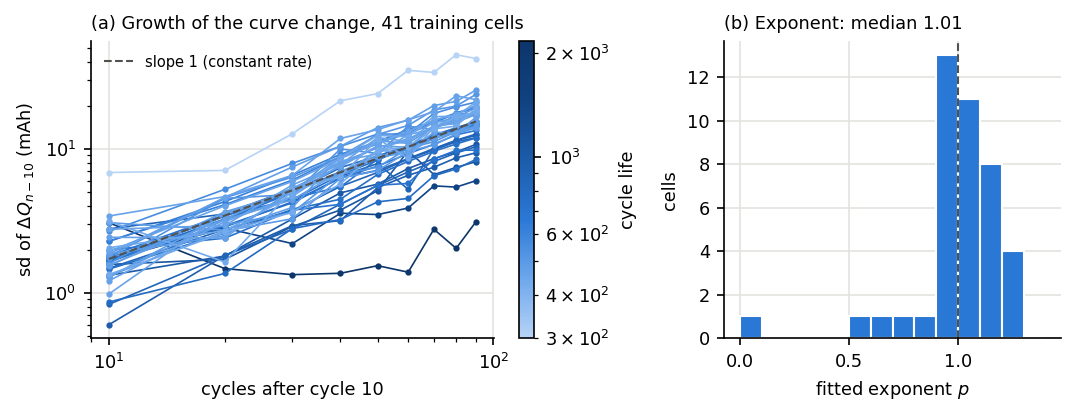
\includegraphics[width=\columnwidth]{fig_p3_traj}
  \caption{(a) Amplitude of $\Delta Q_{n-10}(V)$ against the number of cycles
  after cycle 10, for the 41 training cells (log axes). Dashed: slope 1,
  i.e.\ a constant rate. (b) Fitted power-law exponents.}
  \label{fig:p3traj}
\end{figure}

With a constant rate, life is approximately the capacity budget divided by
the rate. End of life is an absolute threshold (0.88\,Ah), so the budget is
$Q_{D,2}-0.88$\,Ah, and the rate is measured by the amplitude of $\dq$:
\begin{equation}
  \texttt{margin\_rate} = \log_{10}\frac{Q_{D,2}-0.88\,\mathrm{Ah}}{\mathrm{sd}\big(\dq\big)} .
\end{equation}
Nothing is fitted inside the feature. Alone it lowers the cross-validated
error of $\log_{10}\mathrm{Var}(\dq)$ by 9\,\% (better in 96\,\% of folds), ranks
the cells better within both batches (Fig.~\ref{fig:p3margin}), and its
fitted slope against $\log_{10}$(life) is 0.79, close to the value of one that
the budget-over-rate picture predicts. Its added information comes mainly from
\texttt{b1} ($t=+5.3$); within \texttt{b2}, whose lives span only 300--527
cycles, it adds none, and its pooled gain overlaps with the batch difference.
It is kept because the fixed physical form beats a model that weights
$\log_{10}\mathrm{Var}(\dq)$ and $Q_{D,2}$ freely (see the F4 subsection
below).

\begin{figure}[t]
  \centering
  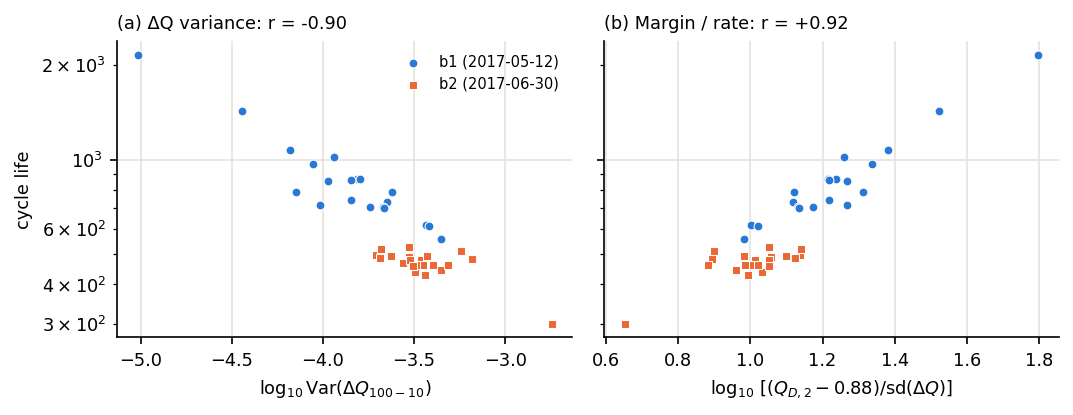
\includegraphics[width=\columnwidth]{fig_p3_margin}
  \caption{Cycle life of the training cells against (a)
  $\log_{10}\mathrm{Var}(\dq)$ and (b) the margin/rate feature.}
  \label{fig:p3margin}
\end{figure}

\subsection{The overhang effect}
In most cells the capacity first \emph{rises} by a few mAh (median 2.6\,mAh over
all batches), peaking around cycle 30--40 in the paper's batches
(Fig.~\ref{fig:p3overhang}a). The paper attributes this to lithium that is
stored in the part of the negative electrode extending beyond the positive
electrode (the overhang) and slowly returns to cycling~\cite{severson2019}.
Two observations matter for $\dq$. First, most of the rise (65--80\,\%) happens
before cycle 10, the start of the $\dq$ window. Second, the returning lithium
appears at the low-voltage end of the discharge (Fig.~\ref{fig:p3overhang}b),
and at \Crate{4} part of it comes out only in the 2.0\,V CV hold, which
\texttt{Qdlin} does not include. As a result, between cycles 10 and 40 the total
capacity rises in 76\,\% of the training cells while $\dq$ is negative on
average in all of them: the plateau shift dominates.

If part of the release happens inside the $\dq$ window, it adds positive charge
at low voltage and partly hides the degradation. A cell with a large rise
\emph{after} cycle 10 should then live shorter than its $\dq$ predicts. This is
what the data show (Fig.~\ref{fig:p3overhang}c): within both batches, given
$\log_{10}\mathrm{Var}(\dq)$, the rise after cycle 10 has a negative coefficient
($t=-3.9$ in \texttt{b1}, $-1.6$ in \texttt{b2}), while the rise before cycle
10 carries much less information ($t=-2.6$ and $-0.7$). The feature
\texttt{overhang\_after10} is the rise of the smoothed capacity (9-cycle rolling
median) from cycle 10 to its maximum within cycles 2--100, in mAh. It is the
only candidate that adds clearly beyond a batch label ($+11$\,\%), and the
result holds for smoothing windows of 5, 9 and 15 cycles. Seven of the 20
\texttt{b1} training cells had a test pause at cycles 12--13; the capacity step
across the pause carries no information ($t=-0.1$), while the gradual rise
after cycle 15 still does ($t=-2.2$), so the signal is not a pause artefact.

\begin{figure*}[t]
  \centering
  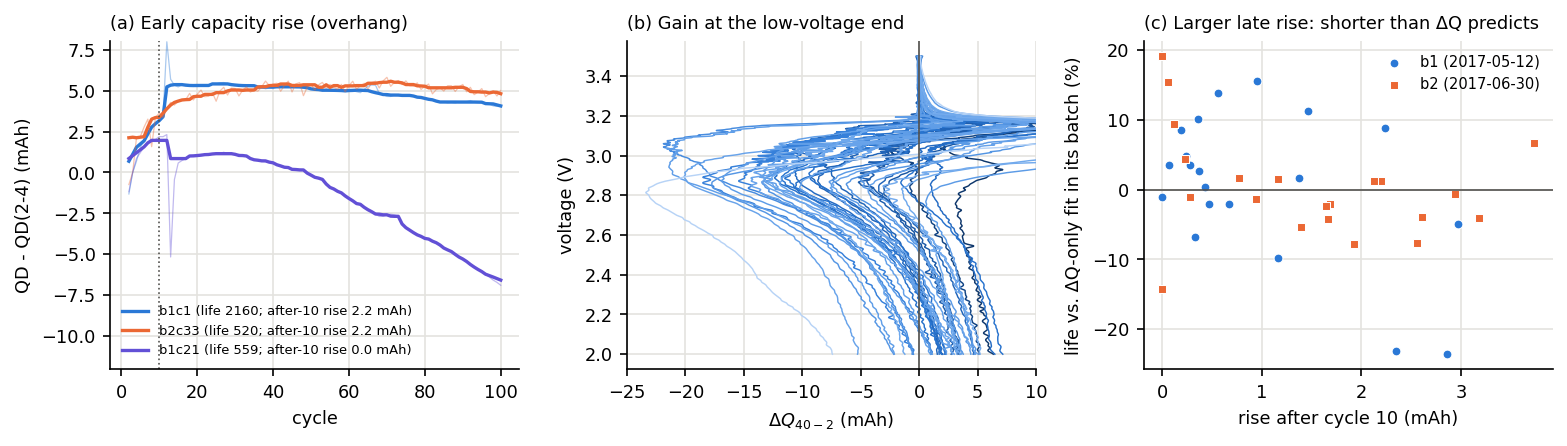
\includegraphics[width=\textwidth]{fig_p3_overhang}
  \caption{(a) Early capacity of three training cells relative to cycles 2--4
  (thin: cleaned data; thick: 9-cycle rolling median); dotted line: cycle 10.
  (b) $\Delta Q_{40-2}(V)$ of the training cells, coloured by cycle life: the
  early gain appears at the low-voltage end. (c) Life relative to a
  $\Delta Q$-only fit within each batch, against the capacity rise after
  cycle 10.}
  \label{fig:p3overhang}
\end{figure*}

The overhang behaviour differs between batches. In \texttt{b3} the rise is
smallest (2.4\,mAh) and earliest (peak near cycle 30); in the standard cells of
the 2018-02-20 batch it is largest (7.0\,mAh), mostly after cycle 10, with a
median peak at cycle 79. The rise therefore depends on the history of each
batch, and the feature may transfer less well than it fits.

\subsection{The F4 feature set}
F4 consists of the two features \texttt{margin\_rate} and
\texttt{overhang\_after10}. Table~\ref{tab:p3sets} compares it with the
paper's sets by nested cross-validation on the training cells, with the
paper's protocol (elastic net tuned by inner cross-validation). The two
features match the nine-feature full model on the log scale and do better in
cycles, without the temperature integral, charge time or IR, which partly act
as batch and policy proxies. Adding them to F3 does not help. With the
overhang feature, \texttt{margin\_rate} also beats $\log_{10}\mathrm{Var}(\dq)$
(0.0509 vs.\ 0.0533, better in 82\,\% of folds) and a model that weights
$\log_{10}\mathrm{Var}(\dq)$ and $Q_{D,2}$ freely (0.0521).

\begin{table}[t]
\centering
\caption{Nested cross-validation on the 40 training cells with a working
temperature probe: RMSE of $\log_{10}$(life) and in cycles; share of outer
folds in which the set beats F2.}
\label{tab:p3sets}
\begin{tabular}{@{}lcccc@{}}
\toprule
Set & Features & $\log_{10}$ & Cycles & $>$F2 \\
\midrule
F1 variance & 1 & 0.0708 & 108 & 22\,\% \\
F2 discharge & 6 & 0.0581 & 94 & -- \\
F3 full & 9 & 0.0510 & 89 & 72\,\% \\
\textbf{F4 physics} & \textbf{2} & \textbf{0.0509} & \textbf{77} & \textbf{78\,\%} \\
F3 + F4 & 11 & 0.0514 & 90 & 70\,\% \\
\bottomrule
\end{tabular}
\end{table}

\subsection{Performance with the paper's model}
F4 was fixed on the training cells before the test sets were used. It was
then evaluated once with the paper's protocol (elastic net tuned by
cross-validation on the training cells, Section~\ref{sec:reproduction}), on
the same splits as the reproduction (\texttt{src/p3\_evaluate.py}). It is not
changed in response to these results. The fitted coefficients on the
standardised features have the signs the physics predicts: $+0.158$ for
\texttt{margin\_rate} (more budget per unit rate, longer life) and $-0.042$ for
\texttt{overhang\_after10} (more hidden release, shorter life).
Table~\ref{tab:p3test} and Fig.~\ref{fig:p3parity} show the results.

\begin{table*}[t]
\centering
\caption{Test performance with the paper's model (elastic net; ordinary least
squares for one feature): RMSE (cycles) / mean absolute percentage error.
Last column: range of test RMSE over 10 cross-validation seeds (primary /
secondary). Rows above the line are the reproduced models of
Table~\ref{tab:repro}.}
\label{tab:p3test}
\begin{tabular}{@{}lccccccc@{}}
\toprule
Feature set & Features & Train & Primary & Primary excl. & Secondary & Seed range \\
\midrule
Variance  & 1 & 104 / 14.1\,\% & 138 / 14.7\,\% & 138 / 13.2\,\% & 196 / 11.4\,\% & -- \\
Discharge & 6 & 69 / 9.2\,\% & \textbf{90} / 12.6\,\% & \textbf{85} / 9.4\,\% & \textbf{167} / \textbf{9.9\,\%} & 89--91 / 167--170 \\
Full      & 9 & 67 / 6.8\,\% & 125 / 11.0\,\% & 122 / \textbf{8.0\,\%} & 220 / 11.2\,\% & 117--128 / 218--222 \\
\midrule
\textbf{F4 physics} & \textbf{2} & 67 / 8.8\,\% & 114 / \textbf{9.9\,\%} & 115 / 9.1\,\% & 170 / 11.1\,\% & 113--116 / 170--171 \\
F3 + F4   & 11 & 65 / 6.7\,\% & 122 / 10.5\,\% & 121 / 7.8\,\% & 205 / 10.8\,\% & 116--124 / 201--207 \\
\bottomrule
\end{tabular}
\end{table*}

\begin{figure}[t]
  \centering
  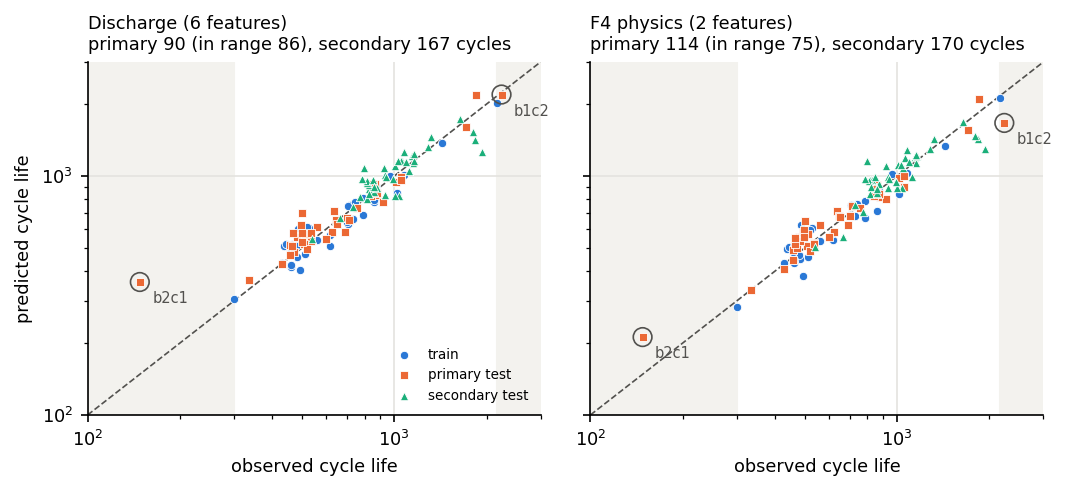
\includegraphics[width=\columnwidth]{fig_p3_parity}
  \caption{Predicted vs.\ observed cycle life for the discharge model and
  F4. Shaded: lives outside the range of the training cells (300--2160
  cycles). Circled: \texttt{b1c2} (2237 cycles) and the anomalous cell
  \texttt{b2c1} (148 cycles).}
  \label{fig:p3parity}
\end{figure}

\textbf{Against the full model} (nine features), F4 is better on every test
split, with two features instead of nine: 114 vs.\ 125 cycles on the primary
set and 170 vs.\ 220 on the secondary set. The secondary set is where the
full model fails, because its temperature integral and charge time partly
encode the training batches (Section~\ref{sec:screen}); F4 does not use
them.

\textbf{Combined with the paper's features.} Adding the two F4 features to
the nine of F3 (11 features, same protocol) improves every split slightly:
primary 125 to 122 cycles, primary inside the training range 71 to 69,
secondary 220 to 205 (Table~\ref{tab:p3test}). These gains are within the
seed and bootstrap uncertainty, except perhaps on the secondary set, and the
combined model remains much worse than F4 alone on the secondary batch (205
vs.\ 170). The fitted weights (Table~\ref{tab:p3coef}) show why. The elastic
net gives \texttt{margin\_rate} the largest weight and moves weight away from
the $\dq$ features, but it keeps the temperature integral and the charge time,
which partly identify the training batches: they fit the two training batches
well, so the penalty has no reason to remove them, and they continue to hurt
on a new batch. It also shrinks \texttt{overhang\_after10} almost to zero, as
part of its information overlaps with those two features. With only two
training batches, a model cannot separate a real effect from a batch label;
adding batch-like features therefore makes it worse on a new batch, which is
the main argument for a small, physics-based feature set.

\begin{table}[t]
\centering
\caption{Elastic-net weights on standardised features (target
$\log_{10}$ life) for the paper's full set (F3), F3 combined with F4, and F4
alone. Dash: feature not in the set.}
\label{tab:p3coef}
\setlength{\tabcolsep}{4pt}
\begin{tabular}{@{}lrrr@{}}
\toprule
Feature & F3 (9) & F3 + F4 (11) & F4 (2) \\
\midrule
\texttt{margin\_rate} & -- & $+0.040$ & $+0.158$ \\
\texttt{overhang\_after10} & -- & $-0.007$ & $-0.042$ \\
$\log_{10}\mathrm{Var}(\dq)$ & $-0.049$ & $-0.030$ & -- \\
$\log_{10}|\min\dq|$ & $-0.040$ & $-0.026$ & -- \\
Charge time, cycles 2--6 & $+0.033$ & $+0.028$ & -- \\
Temperature integral & $-0.029$ & $-0.029$ & -- \\
Capacity, cycle 2 & $+0.025$ & $+0.017$ & -- \\
Minimum IR & $-0.021$ & $-0.017$ & -- \\
IR(100)$-$IR(2) & $0.000$ & $0.000$ & -- \\
Fade slope and intercept & $0.000$ & $0.000$ & -- \\
\bottomrule
\end{tabular}
\end{table}

\textbf{Against the discharge model} (six features) the picture is mixed.
On the secondary set the two are equal (170 vs.\ 167 cycles). On the primary
set F4 has the lower percentage error (9.9 vs.\ 12.6\,\%) but the higher RMSE
(114 vs.\ 90). The difference comes from the two primary-test cells whose
lives lie outside the training range. F4 predicts the anomalous cell
\texttt{b2c1} (148 cycles) much better than any other model (212 vs.\ 360 for
the discharge model), but under-predicts the longest-lived cell \texttt{b1c2}
(2237 cycles) at 1667, which alone causes 58\,\% of its squared error; the
discharge model predicts 2192.

To separate prediction from extrapolation, Table~\ref{tab:p3robust} also
scores the test cells whose observed life lies inside the training range, a
rule that does not depend on any model. It removes these two primary cells
and no secondary cell. It also gives the median and 90th-percentile
percentage error, which need no exclusion. Inside the training range, the
order on the primary set becomes F3 + F4 (69 cycles), full (71), F4 (75),
discharge (86).
A paired bootstrap over the test cells (5000 resamples, identical cells for
all models) shows how much of this is resolved by about 40 test cells:
\begin{itemize}
  \item primary, F4 vs.\ discharge: $-11$ cycles (95\,\% interval $-24$ to
  $+4$; F4 better in 92\,\% of resamples);
  \item primary, F4 vs.\ full: $+5$ ($-18$ to $+33$), no difference;
  \item secondary, F4 vs.\ discharge: $+5$ ($-8$ to $+20$), no difference;
  \item secondary, F4 vs.\ full: $-43$ ($-80$ to $+6$; F4 better in 96\,\%);
  \item secondary, full vs.\ discharge: $+48$ ($+7$ to $+79$), the only
  clearly resolved difference.
\end{itemize}

\begin{table}[t]
\centering
\caption{Robust test scores. In range: test cells whose life lies inside
the training range (300--2160 cycles); this removes \texttt{b1c2} and
\texttt{b2c1} from the primary set and no secondary cell. Med./P90: median
and 90th-percentile absolute percentage error over all test cells.}
\label{tab:p3robust}
\setlength{\tabcolsep}{3pt}
\begin{tabular}{@{}lcccc@{}}
\toprule
& Primary in range & Primary & Secondary & Secondary \\
Set & RMSE / \% & Med. / P90 & RMSE / \% & Med. / P90 \\
\midrule
Constant  & 315 / 27.1 & 27.8 / 59.9 & 511 / 36.1 & 35.4 / 53.6 \\
Variance  & 108 / 12.9 & 12.9 / 25.5 & 196 / 11.4 & 11.2 / 24.5 \\
Discharge & 86 / 9.6   & 8.2 / 17.3  & \textbf{167 / 9.9} & \textbf{7.6} / 20.8 \\
Full      & 71 / 7.5 & \textbf{6.1} / \textbf{16.8} & 220 / 11.2 & 10.0 / \textbf{19.2} \\
F4        & 75 / 8.7   & 7.2 / 17.9  & 170 / 11.1 & 8.7 / 20.0 \\
F3 + F4   & \textbf{69 / 7.3} & \textbf{6.1} / 17.0 & 205 / 10.8 & 9.0 / 19.5 \\
\bottomrule
\end{tabular}
\end{table}

\textbf{What this answers.} Two features built from the physics of the
capacity budget and the overhang perform as well as the paper's six- and
nine-feature models: F4 is the only set close to the best on both test sets,
it beats the full model where that model fails (the secondary batch), and its
test errors change by only 1--3 cycles across random seeds. It does not,
however, clearly beat the discharge model: with about 40 test cells per set,
differences of 10--20 cycles are within the uncertainty. Its one large
weakness is a cell living longer than any training cell. This answers the
first part of RQ3 for the linear model; Phase~4 repeats the comparison with
the other model families, which may extrapolate differently.

\textbf{Caveats.} The features were selected on the training cells after
screening 19 candidates, and the training-set comparison
(Table~\ref{tab:p3sets}) was optimistic: there F4 looked better than the
discharge model, on the test sets it is not. The in-range rule was chosen
after seeing that \texttt{b1c2} dominates the primary RMSE; the official
scores (Table~\ref{tab:p3test}) remain the reference. The within-batch
evidence for both features comes mostly from \texttt{b1}. Finally, the
overhang behaviour of the unseen batch differs from the training batches; if
the explanation above is right, its $\dq$ understates the degradation, which
Phase~5 will test.
